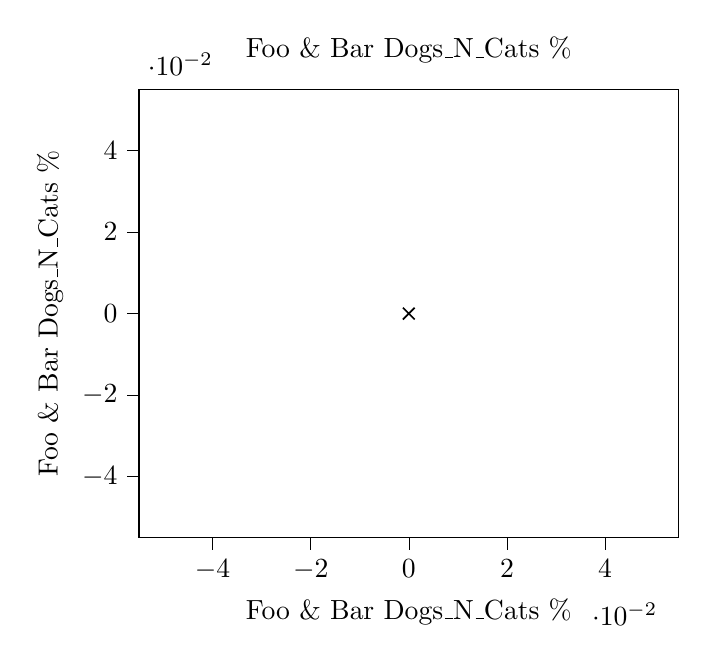
\begin{tikzpicture}

\definecolor{darkgray176}{RGB}{176,176,176}

\begin{axis}[
tick align=outside,
tick pos=left,
title={Foo \& Bar Dogs\_N\_Cats \%},
x grid style={darkgray176},
xlabel={Foo \& Bar Dogs\_N\_Cats \%},
xmin=-0.055, xmax=0.055,
xtick style={color=black},
y grid style={darkgray176},
ylabel={Foo \& Bar Dogs\_N\_Cats \%},
ymin=-0.055, ymax=0.055,
ytick style={color=black}
]
\addplot [semithick, black, mark=x, mark size=3, mark options={solid}, only marks]
table {%
0 0
};
\end{axis}

\end{tikzpicture}
